\documentclass{article}
\def\npart {2}
\def\nterm {LMS Summer School}
\def\nyear {2021}
\def\nlecturer {Various}
\def\ncourse {Colloquia}

\input{header}

\begin{document}
  \maketitle

\section{Markov Numbers and the free group on two generators - Caroline Series.}

We are going to talk about three binary tree and the connections between them.

A Markov number is a solution to,
$$ x^2 + y^2 + z^2 = 3xyz $$
If we set $x=y=z=1$ and that's a solution. Let's not worry about negative solutions as here is another $(-x, -y, z)$. \\

Suppose $x, y_1, z_1$ is a solution you get,
$$ z^2 - 3xy_1z_1 + y_1^2 + z_1^2 = 0 $$
and so $x + x' = 3y_1z_1$. If we have $(x, y_1, z_1)$ we can get $(3y_1z_1 - x, y_1, z_1)$. We could permute any of these. \\

\begin{nthm}
  If we start with a solution, we can carry on permuting, we can get all the solutions,
  $$ (x, y, z) \to (3yz - x, y, z) $$
\end{nthm}
\begin{proof}
  Start with $(x, y, z)$, and let $(1, 1, 1)$ and thenget a load of solutions. We can now put these around the vertices of a binary tree.
  \begin{figure}[!ht]
    \centering
    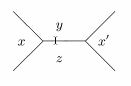
\includegraphics{./figures/L1.1}
  \end{figure}
  and we can do this again, to get a load more solutions,
  \begin{figure}[!ht]
    \centering
    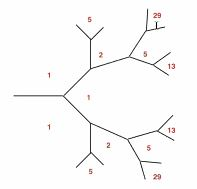
\includegraphics{./figures/L1.2}
  \end{figure}
  Let's now prove that this is all of them, \\
  Say it is special if two of $x, y, z$ are equal. The only special solutions are $(1, 1, 1)$ and $(1, 1, 2)$. Say $x = y$ and then $2x^2 + z^2 = 3x^2z$. Hence $x^2|z^2$ and so $z = kx$ and so $2 + k^2= 3kx$ so $k|2$ and so $k = 1$ or $2$.\\
  \textbf{Step 2:}
  Show that if $(x, y, z)$ is a solution with x < y < z if x' = 3yz - x and x > y > x'.
  \textbf{Step 3:} Take any non-special $x > y > z$ surrounding $V$ and draw it's local tree with arrows. By step 2, there is an outgoing arrow from $x$ to $x'$.
  \textbf{Claim:} The other two arrows at $V$ point to $V$. \\
  This follows from a change of variables, $\xi + \eta+\zeta = 1$ and so again, $\xi + \xi'=1$ and for the other variables. Hence $\xi > \xi'$ and so $\xi > \frac{1}{2}$. But then, $\eta < \frac{1}{2}$ and $\zeta < \frac{1}{2}$, which means that $\eta < \eta'$ and $\zeta < \zeta'$, so the arrows point to $V$.\\
  \textbf{Step 4:} From each non-special vertex there exists
\end{proof}

There is a conjecture that says,
\begin{conjecture}
  Suppose $x > y > z$ and $x > \hat y > \hat z$ are both solutions to Markov equations, then $y = \hat y$ and $z = \hat z$
\end{conjecture}
The conjecture has been checked up to numbers 140 digits long.
\begin{thm}
  The uniqueness conjecture  is truw if the largest number $x$ is the triple of the form $kp^n$ whiere $p$ is prime and $k \le 10^35$
\end{thm}
A simpler proof is given in 2005 about $x$ being a prime power.

\subsection{Free Group on 2 generators}
A free group of two generators, $F_2$, every element is a product of $a$, $a^{-1}$, $b$ and $b^{-1}$. A string of these is called a word, there are no relations expect the identity relation.\\

A generator pair $(\a, \b) \in F_2$ such that every $g \in F_2$ can be written in terms of $\a^{\pi}$ and $\b^{\pm}$. You can get a new generator pair by inverting one generator or by conjugating.

\begin{nthm}
  Every generator pair can be obtained in this way starting from $(a, b)$.
\end{nthm}

A word $w$ which we can find a $v$ such that they are generators are called primitive. We want all of the primitives of our group. We don't want conjuages so we assume that $w$ isn't cyclically reduced.
\begin{align*}
  w = e_1e_2\dots e_n\\
  e_1^{-1}we_1 = e_2e_3\dots e_ne_1
\end{align*}

He shows that after cycliv permutations and cancelling, then if $(\a, \b)$ is a generator we can just and shorten. For Example take, $(ab^2abab^2, ab^2)$ can be reduced to $(a, b)$.\\

We can now put these around our binary tree. Across an edge we have a generator pair.
\begin{figure}[!ht]
  \centering
  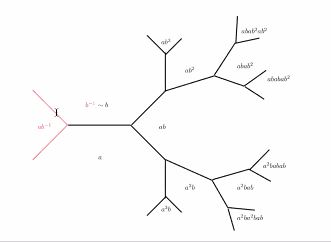
\includegraphics{./figures/L1.4}
\end{figure}
We have generator pairs opposite eachother. We have some fascinating patterns called Sturmian sequences. There is every primite element is represented once and the otheres just have negative exponents.\\

Another proof uses albelianisation of $\Z^2$. If $w \in F_2$ and map it to $\psi (w) = (m, n) \in \Z^2$.We assume everything is commutative and so we can have $\hat w = a^mb^n$. We also note that, $\psi(w^{-1}) = -\psi(w)$ and $\psi(w) = \psi(w')$.\\

\begin{nthm}
  Any primitive element of $F_2$ maps to a relatively prime pair. If $w'$ is another primitive element with $\psi(w') = \psi(w)$, then they are conjuage.
\end{nthm}

What it's telling us that the rationals are an equivilence class around a tree. We shall now look at Farey tree. \\

We say two rationals $\left(\frac{p}{q} \text{ and } \frac{r}{q}\right)$ are neighbours if $ps - rq = \pm 1$. This then means that,
$$ \frac{p}{q} + \frac{r}{s} = \frac{p+r}{q+s} $$
this is called a farey sum and so,
$$ \frac{p}{q} < \frac{p + r}{q + s} < \frac{r}{s} $$
Using the euclidean algorithm it is not hard to show that all positive rationals can be reached this way starting at $\frac{1}{0}$ and $\frac{0}{1}$.
\begin{figure}[!ht]
  \centering
  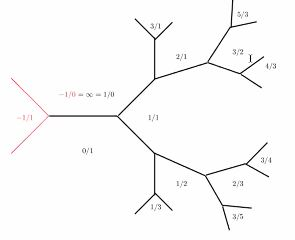
\includegraphics{./figures/L1.5}
\end{figure}
We can just add as we go around and now we have all of the rationals.
We just go around and multiply the trees.\\

Finally we make the connection. Consider elements of $SL(2, \C)$ which all have determinant 1. Now we can consider the trace and it's invariant under conjigation. There are some other polynomial identities. They use the commutator and -2 and we can simplify things nicely,
$$ Tr A Tr B Tr AB = (Tr A)^2 + (Tr B)^2 + (Tr AB)^2 $$
and so we divide by three and get the markov equation. We can also consider $Tr AB^{-1}$ and get that $z + z' = 3xy$. Now it suffices to show that there exists these matrices. Let,
$$ A = \begin{pmatrix}
  1 & 1 \\ 1 & 2
\end{pmatrix} \qquad B = \begin{pmatrix}
  1 & -1 \\ -1 & 2
\end{pmatrix} $$

Now take the tree of generators of the free group and then put them into the Neilson tree and replace $W$ bt $Tr \frac{W}{3}$.\\

\begin{thm}
  The tree of Markov number is found from the three of traces of the above matrices by dividing all entries by 3 and starting the triple $(1, 1, 1)$.
\end{thm}

\subsection{Tree of Traces}
We used the tree of traces and got the special numbers. Why don't any old matrices work? We can sub in and do some generators and find it's trace.

\begin{nlemma}
  Given any triple of complex numbers $(x, y, z)$ there are matrices $A, B \in SL(2, \C)$ so that,
  $Tr A = x$, $Tr B = y$ and $Tr AB = z$
\end{nlemma}
\begin{proof}
  We take,
  $$ A = \begin{pmatrix}
    x & -1 \\ 1 & 0
  \end{pmatrix} \qquad B = \begin{pmatrix}
    0 & \zeta \\ \zeta^{-1} & y
  \end{pmatrix}$$
  where $z = \zeta + \zeta^{-1}$
\end{proof}

and so now we just run through the tree and images of primitive elements. Some questions have been asked is, is the group generated by $A$ and $B$ free? If not, is it discrete?

Are the corresponding groups finite? If we look at the following,
\begin{figure}[!ht]
  \centering
  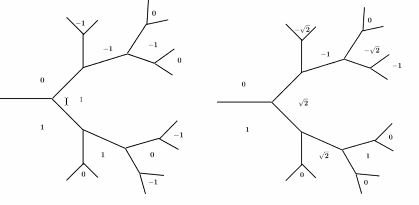
\includegraphics{./figures/L1.6}
\end{figure}

You can see that you won't get past $0$ and $1$ for the first. Then in the second, taking $\sqrt 2$, we can't more values than we have. If a group had generators $0$, $1$ would it be finite? So we now consider $SU(2)$,
$$ M = \begin{pmatrix}
  a & b \\ \overline{a} & \overline{b}
\end{pmatrix} $$
and they are unitary. These basically give us stereographic projections, it didn't preserve distance, but it does for angles. if we rotate our stereographic sphere, we get an angle preserving map. This then gives us $SU(2) \subset SL(2, \C)$. This gives us a mobius transformation. Thn if we consider,
$$ \begin{pmatrix}
  e^{i \frac{\theta}{2}} & 0 \\
  0 & e^{-i \frac{\theta}{2}} \\
\end{pmatrix} $$
We get the trace as just $2\cos \frac{\theta}{2}$. Then out pops $0, 1, \sqrt 2$.

\begin{nthm}
  With one exception, every finite tree is associated to a regular solids, and correspeonds to finite representations to $F_2 \to S(U)$ with finite image. The exception is the dihedral group.
\end{nthm}

The other regular solid is the icosohedron, hence giving the icosohedral group. The sphere is coverd with twenty copies of the a equilateral triangle of angle $\frac{\pi}{5}$. This then moves forward with subgroups generated by rotations of orders $2, 3$ and $5$. So we expect to get a finite tree starting from the values, $2\cos \frac{\pi}{2} = 0$, $2\cos \frac{\pi}{3} = 1$ and $2\cos \frac{\pi}{5} = \omega$ and after some algebra we get that $\omega - \omega - 1 =0$ and hence after some algebra we have finite values.

\section{A Glimpse of Tropical Geometry - Felipe Ricon, QMUL}

Resources - \textit{Introduction to tropical Geometry (Book), First Steps in Tropical Geometry (Article)}

\begin{ndefi}[Tropical Semiring]
  The tropical semiring is,
  $$ \overline{\R} = (\R \cup \{\infty\}, \oplus, \odot) $$
  where,
  $$ \oplus := \min \qquad \odot := + $$
\end{ndefi}

\begin{eg}
  $$ 3 \oplus 5 = 3 \qquad 4 \odot 7 = 11 $$
  $$ \infty \oplus a = a \qquad 0 \odot a = a $$
\end{eg}


$\overline \R$ is an idemoptent remiring as there are no additive inverses.
$$ a \odot (b \oplus c) = a \odot b \oplus a \odot c $$
but things like,
$$ 2 \oplus x = 5 $$
doesn't have a solution in our semiring. But addition is idempotent,
$$ a \oplus a  = a $$
\begin{eg}
  $(x \oplus y)^3 = x^3 \oplus x^2 \odot y \oplus x \odot y^2 \oplus y^3 \equiv x^3\oplus y^3$
\end{eg}

\noindent
Denote $\overline \R [x_1, \dots, x_n]$ the semiring of the tropical polynomials on the variables $x_1, \dots, x_n$.

\begin{eg}
  $f(x) = x^2 \oplus 1 \odot x \oplus 4$
  which then we can plot,
  \begin{figure}[!ht]
  \centering
  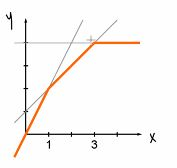
\includegraphics{./figures/L2.1}
  \caption{A graph of $f(x) = (x \oplus 1)\odot (x \oplus 3$}
  \end{figure}

  we note we can factor them as,
  $$ f(x) = (x \oplus 1)\odot (x \oplus 3) $$
  and where we factor it is where the graph bends.
\end{eg}

\newpage
\begin{nthm}[Fundemental Theorem of Algebra]
  If $f(x)\in\overline\R [x]$ has degree $d$ then,
  $$ f(x) \equiv c\odot (x\oplus a_1)^{m_1} \odot (x\oplus a_1)^{m_2} \odot\dots\odot (x\oplus a_r)^{m_r} $$
  where $a_1, \dots, a_r \in \overline\R$ and $m_1 + \dots + m_r = d$
  \begin{figure}[!ht]
  \centering
  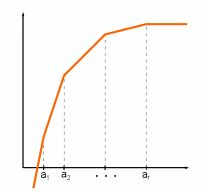
\includegraphics{./figures/L2.2}
  \caption{}
  \end{figure}
\end{nthm}

Any $f(\mathbf{x}) \in \overline\R [x_1, \dots, x_n]$ is the minimum of a load of finite number of affine functions. Then we define,
\begin{ndefi}[Tropical Zero Set]
  $$ \mathcal{V}(f) := \{\mathbf{a} \in \overline\R^n \,|\, \text{ the miniumu of $f(\mathbf{a})$ is attained by at least two terms}\} $$
\end{ndefi}

\begin{figure}[!ht]
\centering
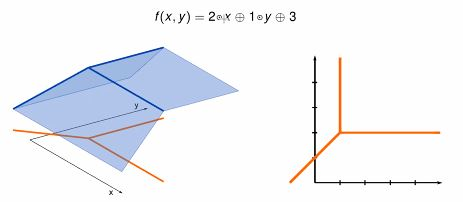
\includegraphics{./figures/L2.3}
\end{figure}

We notice here that instead of points, this time we get some lines where the graph breaks. The tropical zeros are the `bending sets.'\\

\newpage

Now we can consider the following and find the smallest in each region,
\begin{figure}[!ht]
\centering
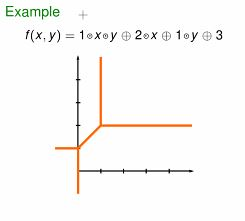
\includegraphics{./figures/L2.4}
\end{figure}

The points where they meet at a point is where they are equal. We have a tropical conic here. Changing the coefficient of the quadratic term from $1 \to -1$ the zero set changes the graph doesn't just flip.\\

Tropical hypersurfaces are `combinatorial' polyhedral complexes with an interesting structure.\\

\subsection{The Tropical Plane}
\begin{minipage}{0.48\textwidth}
  Any two generic tropical lines meets at exactly one point.\\\vspace{30pt}
  \centering
  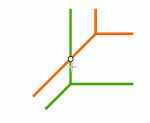
\includegraphics{./figures/L2.5}
\end{minipage}
\begin{minipage}{0.48\textwidth}
  There is unique tropical line going through any two generic points.\\\vspace{30pt}
  \centering
  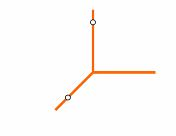
\includegraphics{./figures/L2.6}
\end{minipage}

\begin{minipage}{0.48\textwidth}
  Five points make a conic.\\\vspace{30pt}
  \centering
  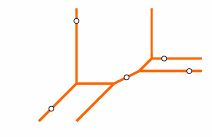
\includegraphics{./figures/L2.7}
\end{minipage}
\begin{minipage}{0.48\textwidth}
  There are no parallel lines in the tropical world. Every collection of lines always intersect once.\\\vspace{30pt}
  \centering
  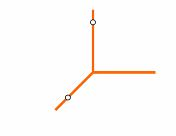
\includegraphics{./figures/L2.6}
\end{minipage}

\newpage
\subsection{Why Tropical Geometry}
Let $K$ be an algebraically closed field with a valuation map: $\text{val}: K \to \overline\R$, that is,
$$ \val(a \cdot b) = \val a \odot \val b \quad \val (a + b) \ge \val a \odot \val b \quad \val a = \infty \iff a = 0  $$

\begin{ndefi}[Trivial Valuation]
  $$ \val x = \begin{cases}
    0 & \text{if $x\ne 0$ }\\
    \infty & \text{otherwise}
  \end{cases} $$
\end{ndefi}

\begin{eg} Here are some fields with evaluations,\\
  \begin{itemize}
    \item Let $K = \C$ and with the trivial evaluation.
    \item $K = \overline\Q$ with the p-adic evaluation.
    \item $K = \C\{\{t\}\}$ the field of Pulseux series; a formal power series of the form,
    $$ a = c_0t^{r_0} + c_1t^{r_1} + \dots + c_kt^{r_k} + \dots$$
    with $c_i \in \C$ and $r_0 < r_1 < \dots$ rational numbers with a common denominator and valuation $\val a = r_0$.
  \end{itemize}
\end{eg}

\noindent
One can tropicalise any $F \in K[x_1, \dots, x_n]$ to $\trop(F) \in \overline\R [x_1] $ by substituting,
$$ + \to \oplus \quad \cdot \to \times \quad f \to \val f $$

\noindent
Suppose $V$ be the zero locus of an ideal $J \subset K[x_1, x_2, \dots, x_n]$. Consder an ideal,
$$ \trop(J) := \langle \trop(F) := F \in J \rangle \subset \overline\R[x_1] $$
The tropicalisation of $V$ is,
$$ \trop := \bigcap_{f \in \trop J} \mathcal{V}(f) $$

\begin{eg}
  Let K= \{\{t\}\} and let $J = \langle x - t \cdot y + q\rangle \subset K[x, y]$ and $V = \{x - t \cdot y + 1 = 0\} \subset K^2$.
  Then we just take the functions and do the tropicalisation,
  \begin{figure}[!ht]
  \centering
  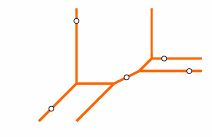
\includegraphics{./figures/L2.7}
  \end{figure}
  and then we get a tropical line. Which is, $\trop V$.
\end{eg}

\newpage
Tropical varieties preseves many invariants of their defining algebraic varieties. It preserves degrees and genus, which is really nice as you can get rid of singularities. We can use the tropicalisation to make sense of some thing yucky and complicated. The tropical degree is the number of rays doing in the imporant directions.\\

\begin{figure}[!ht]
\centering
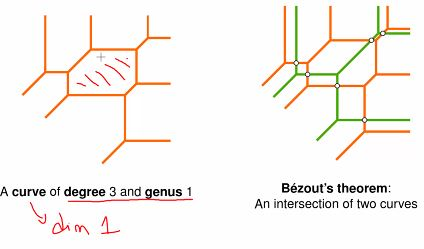
\includegraphics{./figures/L2.9}
\end{figure}


Tropical Geometry has another Bezout's Theorem (which is the same as normal geometry), we can use this with tropical varieties to see the points of intersections. In the diagram above, we have an orange degree 3 and green degree 2 curve. Then we have six intersections.


\begin{ndefi}[Severi Degree]
  The severi degree $N^{d, \delta}$ of $\C\P^2$ is the number of plane curves of degree $d$ and $\delta$ nodal singularities passing through $\frac{(d+3)d}{2}-\delta$ generic points.
\end{ndefi}

\begin{eg}
  \begin{itemize}
    \item $N^{2,0} = $ number of smooth conics through five points. This is one.
    \item $N^{2,1} = $ number of 1-nodal conics through four points. This is three.
    \begin{figure}[!ht]
    \centering
    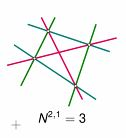
\includegraphics{./figures/L2.10}
    \end{figure}
    \item  $N^{3,1} = $ number of 1-nodal cubics through eight points. This is twelve.
  \end{itemize}
\end{eg}

\begin{nthm}[Mikhalkin 2005]
  Severi degree can be computer tropically
\end{nthm}

\begin{nthm}[Formin-Mikhalkin 2010, conj. Francesco-Itzykson 1994]
  For a fixed $\delta$ thre is a polynomial $N_\delta (d)$ such that for all $d \ge 2\delta$,
  $$ N^{d,\delta} = N_\delta (d) $$
\end{nthm}

\begin{eg} Here are some people that have solved certain values of this problem,
  \begin{itemize}
    \item Steiner 1848: $N^{d,1} = 3(d - 1)^3$
    \item Cayley 1863: $N^{d,2} = \frac{3}{2}(d - 1)(d-2)(3d^2 - 3d - 11)$
    \item Roberts 1867: $\delta = 3$
    \item Vainsencher 1995: $\delta = 4, 5, 6$
    \item Keiman-Piene 2001: $\delta = 7,8$
    \item Block 2010: $\delta = 9, 10, 11, 12, 13, 14$
  \end{itemize}
  \begin{figure}[!ht]
  \centering
  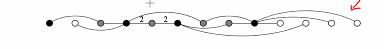
\includegraphics{./figures/L2.11}
  \end{figure}
\end{eg}

Similar approaches have succeeded in the study of Severi degree $N^{\Delta, d}$ of more general toric surfaces, double Hurwitz numbers $H_g(\l, \mu)$, Welshinger invariants $W_d$, ...


\section{Cluster Algebras, Quivers mutations and triangulated surfaces - Anna Felikson}

\textbf{Further Reading:} \href{http://www.math.lsa.umich.edu/~fomin/cluster.html}{Clusted Algebra Portal}\\

\subsection{Cluster Algebra}
Very new, twenty years ago. It go connected to many many different areas of Maths.

\begin{nthm}[Ptolemy Theorem]
  ef = ac + bd on a cyclic quadrilateral
\end{nthm}


\begin{ndefi}[Quiver]
  A quiver is a direct graph without loops and 2-cycles.
\end{ndefi}

\begin{ndefi}[Mutation]
  A mutation , $\mu_k$ of quiver:
  \begin{itemize}
    \item reverse all arrows incident to $k$
    \item for every path through $k$ with  and $p, q > 0$, do:
    \[\begin{tikzcd}
    	& \bullet &&&& \bullet \\
    	&& {} && {} \\
    	\bullet && \bullet && \bullet && \bullet
    	\arrow["p", from=3-1, to=1-2]
    	\arrow["r", from=3-3, to=3-1]
    	\arrow["q", from=1-2, to=3-3]
    	\arrow["p"', from=1-6, to=3-5]
    	\arrow["{pq-r}"', from=3-5, to=3-7]
    	\arrow["q"', from=3-7, to=1-6]
    	\arrow["{\mu_k}", shift right=2, squiggly, from=2-3, to=2-5]
    \end{tikzcd}\]
  \end{itemize}
\end{ndefi}

\begin{eg}
  \begin{figure}[!ht]
  \centering
  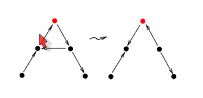
\includegraphics{./figures/L3.2}
  \end{figure}
  \begin{figure}[!ht]
  \centering
  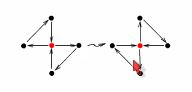
\includegraphics{./figures/L3.3}
  \end{figure}
\end{eg}

If we have a quiver with six arrows, we can mutate however we want and do it in all directions and then we get new quivers and we can mutate again.\\

$$ \text{Iterated mutations} \longrightarrow \text{many other quivers} $$
$$ Q \longrightarrow \text{It's mutation class} $$

\begin{property}
  $\mu_k \circ \mu_k (Q) = Q$ for any quiver $Q$.
\end{property}

We get a regular graph.
\newpage
\begin{ndefi}[]
  A quiver is of finite mutation type if its mutation class contains finitely many quivers
\end{ndefi}

\begin{question}
  Which quivers are of finite mutation type?
\end{question}

Quick answer, not many.

\begin{nlemma}[]
  If $Q$ is connected $|Q| \ge 3$ and $Q$ contains arrow $\longrightarrow$ with $p > 2$, then $Q$ is mutation finite.
\end{nlemma}

if $q > r > 0$ and $p > 2$ , then you can make each step bigger and bigger at every step.
\begin{figure}[!ht]
\centering
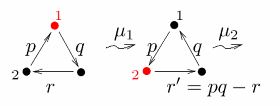
\includegraphics{./figures/L3.5}
\end{figure}

\subsection{Cluster Algebra}

\begin{ndefi}[Seed]
  A seed is a pair $(Q, \mathbf{u})$, where,
  \begin{itemize}
    \item $Q$ is a quiver with $n := |Q|$ vertices.
    \item $\mathbf{u} = (u_1, \dots, u_n)$ is a set of rational functions.
  \end{itemize}
  Initial seed is $(Q_0, \mathbf{u}_0)$\\
  Seed mutation: $\mu_k(Q, \mathbf{u}) = (\mu_k(Q), \mathbf{u}')$ where,
  $$ u_k' = \frac{1}{u_k}\left( \prod_{i \to k} u_i + \prod_{k \to j} u_j \right) $$
  if $u_i' = u_i$ if $i = k$\\
  \textbf{Cluster Variable:} A function of seeds
  \textbf{Cluster Algebra:} An alegbra with seeds and $+$ and $*$.
\end{ndefi}

We can link this to Markov Equation using the Markov quiver.


By definition
$$ u_i = \frac{P(x_1, \dots x_n)}{R(x_1, \dots, x_n)} $$
where $P$ and $R$ are polynomials.

\begin{nthm}[Laurent Phenomenon]
  $R$ is a monomial, $R = x_1^{d_1}x_2^{d_2}\dots x_n^{d_n}$
\end{nthm}

\begin{nthm}[Positivity]
  $P$ has positive coefficients.
\end{nthm}

\begin{ndefi}[Finite]
  A cluster algebra is of finite type, so contains finitely many cluster variables.
\end{ndefi}

\begin{nthm}[]
  A cluster algebra $\mathcal{A}$ is of finite type iff $Q$ is mutation equivilent to an orientation of a Dynkin diagram, $A_n, D_n, E_6, E_7, E_8$.
\end{nthm}

Dynkin diagrams describe: finite reflection group, semisimple Lie Algebras, surface singularities...

A cluster algbra $\mathcal{A}(Q)$ is of finittype if $Q$ is of finite mutation type.

\begin{figure}[!ht]
\centering
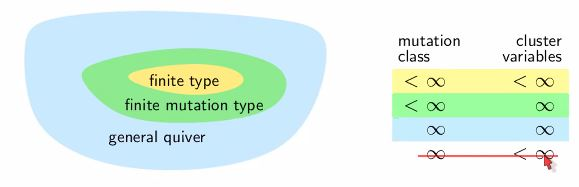
\includegraphics{./figures/L3.6}
\end{figure}

\begin{eg}
  \begin{itemize}
    \item $n= 2$
    \[\begin{tikzcd}
	\bullet & \bullet
	\arrow[from=1-1, to=1-2]
\end{tikzcd}\]
    \item Quivers arising from triangulated surfaces.
    \item Finitely many except that.
  \end{itemize}
\end{eg}

To create a quiver from a triangulation

\begin{figure}[!ht]
\centering
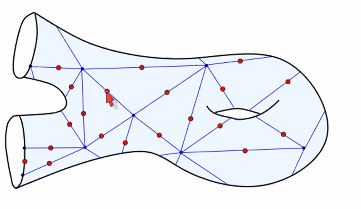
\includegraphics{./figures/L3.7}
\caption{}
\end{figure}

Every edge of the triangulation, is a vertex of the quiver. Two eges of one triangle is an arrow of the quiver. This allows us to mutate by just rotating the diagonal.

\begin{remark}
  $Q$ from a triangulation $\implies$ weights of arrow $\le 2$.
\end{remark}
as every arc lies at most in two triangules.

\begin{nthm}[Hatcher 1991]
  Every two triangulations of the same surface are connected by a sequence of flips.
\end{nthm}

\begin{ncor}
 \begin{enumerate}
   \item Quivers from triangulations of the same surface are mutation-equivalent (and form the whole mutation class).
   \item Quivers from triangulations are mutation-finite.
 \end{enumerate}
\end{ncor}

\begin{question}
  What else is mutation finite?
\end{question}

Any triangulated surface can be glued of,
\begin{figure}[!ht]
\centering
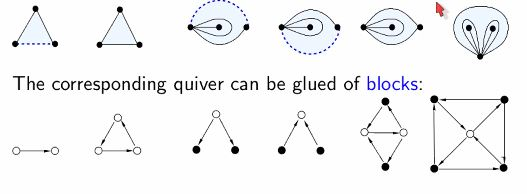
\includegraphics{./figures/L3.8}
\caption{}
\end{figure}

\begin{prop}
  \{$Q$ is from triangulation\} $\iff$ \{$Q$ is block-decomposable\}
\end{prop}

\begin{question}
  How to find all mutation-finite but not block-decomposable quivers
\end{question}

\textbf{Interlude:} How to classify hyperbolic space,\\
\begin{enumerate}
  \item They correspond to some polytopes.
  \item Combinatorics of these polytopes are described by:
  \begin{enumerate}
    \item subdiagrams corresponding to finite objects
    \item minimal subdiagrams corresponding to infinite objects.
  \end{enumerate}
\end{enumerate}

\textbf{Idea:} Classify minimal non-decomposable quivers!

\begin{nlemma}[]
  If $Q$ is minimal non-decomposable quiver then $|Q| \le 7$
\end{nlemma}

\begin{nlemma}[]
  If $Q$ is a minimal non-decomposable mutation-finite quiver, then it is equivilent to one of,

\end{nlemma}


\begin{nthm}[]
  Let $Q$ be a connected quiver of finite mutation type:
  \begin{itemize}
    \item $|Q| = 2$
    \item $Q$ is obtained from a triangulated surface.
    \item $Q$ is mutation-equivalent to one of the following,
    \begin{figure}[!ht]
    \centering
    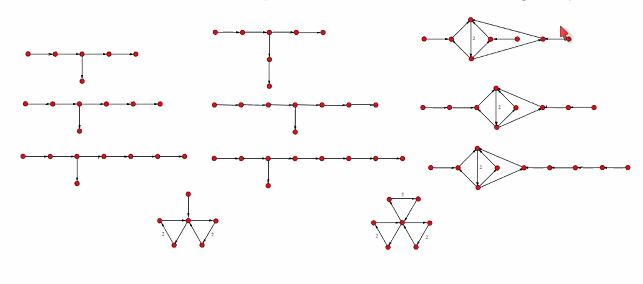
\includegraphics{./figures/L3.9}
    \end{figure}
  \end{itemize}
\end{nthm}

\begin{proof}
  Terrible and technical. It follows the same step as classifications of tesselations.
\end{proof}

\section{Countability, Groups, Subgroups and Finiteness Properties - Ian Leary}

There are three theorems from 1949, 1961 and 2018. They are all of the form,
Which groups arise as subgroups of...\\

\begin{nthm}[Higman Neumann Neumann, 1949]
  Every countable group embeds in a 2-generator group.
\end{nthm}

\begin{nthm}[Higman, 1961]
  A finitely generated group embeds in a finitely presented group iff it is recursively presented.
\end{nthm}

\begin{nthm}[Ian J Leary, 2018]
  Every countable group embeds in an almost finitely presented group.
\end{nthm}


\subsection{Countability}
Infinite sets have the same cardinality if there is a bijection between them. A countable set is one that is bijective with $\N$.\\
Cantor showed that the powerset of any set $X$ is bigger than $X$.

\begin{nthm}[Cantors Diagonal Argument]
  There is no bijection between $f : X \to \mathcal{P}(X)$
\end{nthm}
\begin{proof}[Cantors Diagonal Argument]
  Given $f$, define,
  $$ Y = \{x \in X : x \notin f(x)\} $$
  For any $x \in X$, $Y \ne f(x)$, because $x \in Y \triangle f(x)$
\end{proof}

We can do aleph numbers and talk about cardinality.
$$ 2^{\aleph_0} = |\mathcal{P}(\N)| $$
which is just $|\R|$.

\subsection{Transendental}
An algebraic number is $\l \in \C$ that is a root of $f(x) \in \Q[x]$. A transendental number is non-algebraic. Open problem: If there a $f(x, y) \in \Q[x, y] \ne 0$ such that, $f(e, \pi) = 0$. Are they transendentally independent?

\begin{ndefi}[Louville transendental]
  $$ \sum_{n>0}{ \frac{1}{10^{n!}} } $$
\end{ndefi}

\begin{nlemma}[]
  If $\l \in \R$ is algebraic and not rational there are $K, m > 0$, so that for all large $q$,
  $$ \left| \l - \frac{p}{q}  \right| \ge \frac{1}{Kq^m} $$
\end{nlemma}

If $\a$ is algebraic, then pick $f(x)$ with $f(\a) = 0$, then if $\a$ is a repeated root of $\a$, then consider $f'(x)$ instead. So wlog, consider $\a$ a root with multiplicity one. Also by considering multiplying by common denominator, let $f(x) \in \Z[x]$, then $f(\a) = 0$ and $f'(\a) \ne 0$.\\

Let $m = \deg f(x)$, then for $\frac{p}{q}$ close to $\a$,
$$ f\left( \frac{p}{q} \right) = 0 \quad \left| f\left( \frac{p}{q} \right) \right| = \frac{1}{q^m}$$

Then if we draw the graph of $f(x)$, we shall get a straight line,

\begin{figure}[!ht]
\centering
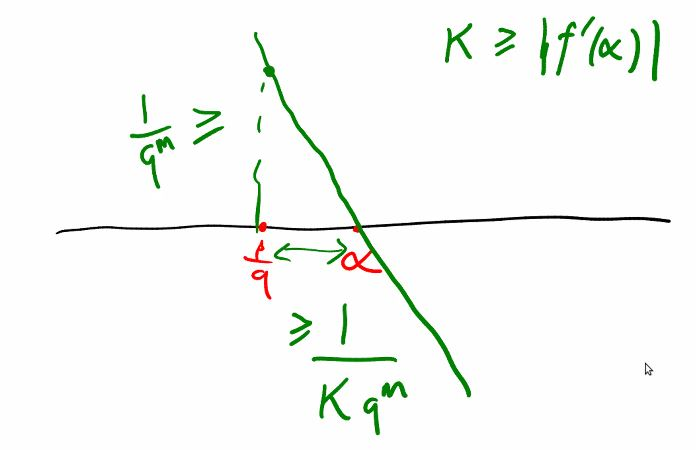
\includegraphics{./figures/L4.1}
\end{figure}

Cantors Ageument:\\
There are only countably many polynomials $f(x) \in \Q[x]$, each with finitely many roots.

\subsection{Countable Groups}

A subset $S$ of a group $G$ generates $G$ if no proper subgroup contains $S$. equivalently, all elements of $G$ can be written as products of elements of $S$ and their inverses. $T \subset \N$,
$$ \bigoplus_{p\in T} C_p $$
$G$ is finitely generated if some finite $S$ generates.

\begin{ndefi}[Finitely Presented]
  $G$ is finitely presented if $G$ is finitely generated and the is a finite list of equations,
  $$ w_1(a, b, c, \dots) = 1 \quad w_2 = 1 \quad\dots $$
\end{ndefi}

\begin{eg}
  The free group $\F_2$, $\langle a, b : \rangle$
  \begin{figure}[!ht]
  \centering
  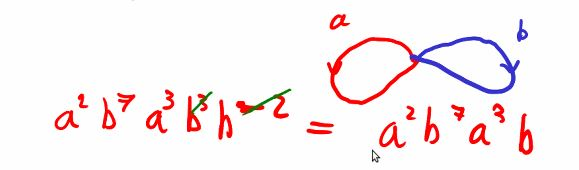
\includegraphics[width=0.3\textwidth]{./figures/L4.2}
  \end{figure}
  You can make the universal cover of the tree,
\end{eg}

\begin{eg}
  The free albelian group $\Z^2$,
  $$ \langle a, b : aba^{-1}b^{-1} = 1 \rangle $$
  \begin{figure}[!ht]
  \centering
  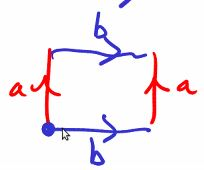
\includegraphics[width=0.1\textwidth]{./figures/L4.3}
  \end{figure}
\end{eg}

\begin{nthm}[B H Neumann]
  There are $2^\aleph_0$
\end{nthm}

\begin{proof}[Proof 1]
  In the group $\prod_{n \ge 2} A_{2n+1}$ and look at,
  $$ ((1, 2, 3), (1, 2, 3), \dots) $$
  and,
  $$ ((1, 2, 3, 4, 5), (1, 2, 3, 4, 5, 6, 7), \dots) $$
  This group has $A_n$ as quotient iff $n \ge 5$ and odd.
\end{proof}

\begin{proof}[Proof 2 - Small Cancellation]
  Given a disk $D$ made out of triangles,
  $$ \sum_{V \in D^\circ} [6 - d(v)] + \sum_{v \in \delta D} [4 - d(v)] = 6 $$
  This has consequences for group presentations in which the relators can only overlap in short pieces.
\end{proof}

A group presentation is $C'\left(\frac{1}{6} \right)$ if the the length of any common piece of two relators less than $\frac{1}{6}$ of the length of each of them.

\begin{figure}[!ht]
\centering
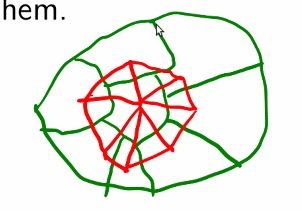
\includegraphics[width=0.2\textwidth]{./figures/L4.4}
\end{figure}

You can nicely cancel things down. If $w = 1$ in a group, with a $C'\left( \frac{1}{6}\right)$ presentation, then $w$ contains more than half a relator as a subword.


For any $S \subset \N$, the words,
$$ a^nb^nc^n \dots m^n \quad n \in S$$
These are going to satisfy the $C'\left( \frac{1}{6} \right)$


There are uncountably many non-isomorphic groups.
$$ G(S) = \langle a, \dots, m : a^nb^nc^n \dots m^n = 1 \quad n \in S \rangle $$

$$ G(S) \times C_{13} $$ % may be fish
None of these are isomorphisms because $S \subset T$ and,
$$ G(S) \to G(T) $$

\begin{nthm}[HNN]
  Every countable group embeds in a 2-generator group
\end{nthm}

For any group $H$ and for any isomorphism $f ; A \to B$, $A, B \le H$, there is a group $G$ and an element $t \in G$ so that $H \le G$ and for $a \in A$, $ta^{-1}t = f(a)$
\begin{figure}[!ht]
\centering
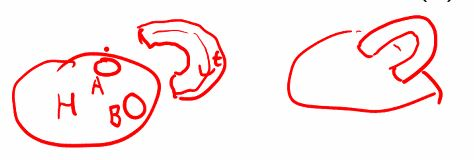
\includegraphics[width=0.3\textwidth]{./figures/L4.5}
\end{figure}
This is a HNN extension.

We take the group and add the two loops, then we can find a free group on countably many generators. We can create two subgroups, one with $a$'s and the other $b$'s. Now we change the elements slightly, we add on just elements of the group and we still have a free group, so then we add the HNN extention and glue the blob on, we only two generators for the whole group.
$$ {\color{green} g_3 } = {\color{green} b^3 a b^{-3}a^3 b a^{-3} } $$

There are only countably many finitely presented group and each have countably many elements and hence pairs of groups. There are only countably many 2-generator groups. Which ones fit?

\begin{nthm}[]
  Higman
\end{nthm}

$G$ is recursively presented if there is an algeothm that it would print out all of the words of $w = 1$.

\begin{proof}[]
  One way around is a lot easier. If $G \le H$ with $H$ finitely presented.\\
  Higmans Rope Trick reduces to a question about $\F_2$. Then you go from $\F_2$ to $\N$
  $$ e \to 0 \qquad a \to 1 \qquad b \to 2 \qquad b^{-1} \to 3 \qquad a^{-1} \to 4 \qquad abba \to 1221 $$
  Recursively enumerable subsets of $\N$ can be coded by in finitely presented groups.
\end{proof}


A family of groups parametrised by nice spaces $L \to BB_L$. Then it was generalised to $G_L(S)$ and then you get finitely many of them. All of these tricks work again, then hence you can encode naturals. All subsets of $\N$ can be coded up in almost finitely generated groups.

The elements of $\Z G$ are finite sums such that
$$ n_1g_1 + \dots + n_kg_k $$
with $g_i \in G$ and $n_i \in \Z$ and we can do,
$$ ng \cdot mh = nm(gh) $$
\begin{eg}
  If $G = \langle a \rangle$, then,
  $$ \Z G = ???$$
\end{eg}

Then we have a ring homomorphism called the augementation ideal and then we can say that $G$ is almost finitely presented if $I_G$ is finitely presented as a $\Z G$-module.

\section{Gradient flows in Differential Geometry}

Given $E : \R^2 \to [0, \infty)$, $u \in \R^2$ and a direction $v$ we know that,
$$ \frac{d}{dt}_{t=0} E(u + tv) = \nabla E(u) \cdot v \ge  -\|\nabla E(u) \|\cdot \|v\| $$
with `=' if and only if $v$ is in the direction of $-\nabla E(u)$. If we evolve an initial state we can then take a minimal point and show that,
$$ \nabla E(u_\infty) = 0 $$

\subsection{Classical Geometry}
Consider a two-dimensional $\Sigma$ in $\R^3$.
\begin{itemize}
  \item Is there a shortest connection between any two points $p_1, p_2 \in \Sigma$? Is there a shortest closed curve in any homotopy class?
  \item How can we change a given curve $\gamma$ into a curve with minimal length, or more generally into a critical point of the length functional? i.e. a geodesic.
\end{itemize}

\noindent
We can now consider minimal surfaces. If we are given some boundary surface in space. Can we find some sort of surface where the boundary is the boundary surface? This is called the plateau problems. This is because it's basically described using soap film.

\noindent
So can we change any given surface into a minimal surface, by leaving the boundary as it is?

\subsection{Harmonic Maps}
Given a domain $M$ and a target $N$, we can consider the dirichlet energy,
$$ E(u) := \frac{1}{2}\int_M |\nabla u|^2 \qquad \text{ of maps $u : M \to N$}$$
We want some sort of domain into some sort of target.\\

Critical points of $E$ are called the harmonic maps and special cases include,
\begin{itemize}
  \item harmonic functions, i.e. solutions to $u_{xx} + u_{yy} =0$
  \item closed geodesics respectively for geodesics with given endpoints.
  \item parameterisation of minimal surfaces, if a harmonic map has the additional propertly that it preserves angles. (i.e. it is conformal)
\end{itemize}

\subsection{Gradient flows of length}
\begin{itemize}
  \item Curve shortening flow,
  $$ \partial_t \gamma = \kappa \vec n $$
  \item Mean curvature flow,
  $$ \partial_t X = - H\vec n $$
  where $H = \kappa_1 + \kappa_2$
  \item Harmonic Map Flow, evolving map $u : M \to N \to \R^m$ %embedding
  by,
  $$ \partial_t u = -\nabla (u) = \Delta u + A(u)(\nabla u, \nabla u) $$
  where $A$ is the second fundemental form that describes how the target $N$ is curvd in the surrounding euclidean space,
  \item $N = \R^n$, we have the heat equation
  \item $N = S^2$ : $\partial_t - \Delta u = |\nabla u|^2 u$
\end{itemize}

\subsection{Properties of gradient flows}
If we hope to find minimisers / critical points of a function $E$ as $t \to \infty$ we need to ask,
\begin{enumerate}
  \item Do the solutions of the gradient flows exist for all time?
  \item If so, do they converge as $t \to \infty$
  \item If so, is the limit a minimiser or at least a critical point.
\end{enumerate}

For model case of $E : \R^2 \to [0, \infty)$ solutions exist for all times thanks to picard's existence theorem. In general, we have non-linear PDEs. We can use Lebesgue intgration and Functional Analysis. Some flows may have `weak solutions' though.

\subsubsection{Convegence}
Consider $\partial_t u = -\nabla E(u)$
for $t \in [0, \infty)$ and we can recall,
\begin{align*}
  \frac{d}{dt} E(u) = \|\nabla E(u)\|^2 \\
  &= -\|\partial_t u\|^2
\end{align*}
and so we can integrate,
\begin{align*}
  \int_0^\infty \|\partial_t u\|^2 &= E(u_0) - \lim_{t \to \infty} E(u(t))
\end{align*}

and so we can't escape to infinity in finite time.
\begin{align*}
  \|u(T) - u(0)\| &\le \int_0^\infty \|\partial_t u\| \cdot T\\
  &\le \left| \int_0^\infty \partial_t u \right|^{\frac{1}{2}}T^{\frac{1}{2}}\\
  &\le E(u_0)^{\frac{1}{2}}T^{\frac{1}{2}}
\end{align*}
But we can have $\int_0^\infty \|\partial_t u\|= \infty$

If $u(t) \to u_\infty$ as $t \to \infty$ then $\nabla E(u_\infty) = 0$. So, do we get convergence?
\begin{itemize}
  \item $\|u(t)\| \to \infty$ as $t \to \infty$. Then this can be realised as we let the infinimum be at infinity. However, this isn't what an energy should be doing. Energy punishes large norms in the right norms.
\end{itemize}

Many energies are coecive wrt the right norm.
$$ E(v) \to \infty \qquad \|v\|\to\infty $$
\begin{eg}
  For the harmonic map,
  $$ E(u) = \frac{1}{2}\int |\nabla u|^2\,dx $$
  for this the right space is $H^1 = W^{1, 2}$ we have sobolev space.
  $$ H^1 = \{F : M \to N : f \text{ if weakly differentiable and } \int|\nabla f|^2 +|f| < \infty\} $$
  $E$ is coercive wrt a norm if $M$ and $N$ are bounded. For analysis with $H^1$, but natural $\nabla$ flow is definite wrt a $L$-innerproduct, i.e.
  $$ \int \nabla E(u) \cdot h = \frac{d}{dt}E(u + th) = \langle \nabla E(u) , h \rangle_{L^2}$$
\end{eg}

If $E$ is coercive and nice, does that imply convergence? Nice really means analytic and so we then get convergence in,
\begin{itemize}
  \item finite dimensions
  \item for gradient flows such as the harmonic map flow if no singularities form.
  \item also if singularity formations.
\end{itemize}

Let's consider a hill, an analytic hill, then a ball or drop of water will converge to a minimiser, a ring of minimal points. How do we take this hill interesting? Well we get some goats. Hills with goat tracks are not always analytic. The goats will dip the earth and make little windings. The problem now is that the drop of water will flow around and assymptote to the minimisers.

\begin{nthm}[Lojasiewicz, 1962]
  If $E : \R^n \to \R$ is analytic, then:
  $$ \forall u^*, \nabla E(u^*) = 0 \exists \e > 0, \gamma \in [\frac{1}{2}, 1], |E(u) - E(u^*) \le \|\nabla E(u)\| \forall u, \|u - u^*\| < \e| $$
\end{nthm}
Then Simon in 1982, adapted this theorem for $E(u) = \int_\Omega L(u, \nabla u, x) dx$ which is analyticall convex. The current research is about Lojest. got settings with singulatirites and changing topologies.
\begin{itemize}
  \item Topping ('04) HMF : $S^2 \to S^2$
  \item Colding-Minisozki `15 MCF
  \item Melanie HMF and H-surfaces.
\end{itemize}

Now let's prove this theorem which stops the annoying problem with infinite length.

\begin{claim}
  Suppose $\partial_t = -\nabla E(u)$ is such that $\hat E(u) := E(u) - \lim_{T \to \infty} E(u(T))$ satisfies,
  $$ \hat E(t)^\g \le \|\nabla E(u(t))\| $$
  with $\g \in [\frac{1}{2}, 1]$. Then,
  $$ \int_0^\infty \|\partial_t u\| < \infty $$
\end{claim}
\begin{proof}
  So consider,
  $$ -\frac{d}{dt} \hat E = \|\nabla E(u)\|^2 = \|\partial_t u\|\cdot \|\nabla E\| $$
  so,
  $$ -\frac{d}{dt} \hat E^{1-\g} = (1 - \g) \hat E^{-\g}\|\nabla E\|\cdot \|\partial_t u\| \ge (1 - \g)\|\partial_t u\| $$
  and then we can integrate and get the conclustion,
  $$ \int_{+}^\infty \|\partial_t u\| \to 0 $$
  so we get (some) convergence.
\end{proof}

If $\g > \frac{1}{2}$ we get that it diverges, but if $\g = \frac{1}{2}$ we get exponential convergence


\end{document}
